% !Mode:: "TeX:UTF-8" 

\BiChapter{图表公式排版}{Figures, Tables and Equations}

虽然本模板不涉及 \LaTeX{} 的详细使用方法,但是为了方便大家使用本模板撰写学位论文,本章对论文写作中经常用到的{\hei 图、表、公式}等内容的排版方法做一个简单的介绍。

%=========================================================================================
\BiSection{图}{Figures}

插图须紧跟文述。在正文中,一般应先见图号及图的内容后再见图,一般情况下不能提前见图,特殊情况须延后的插图不应跨节。

\LaTeX{} 中所使用的图片通常为~PDF~格式,图片应大小适宜,主题明确,层次清楚,金相组织类的照片一定要有比例尺。

图应具有“自明性”,即只看图、图题和图例,不阅读正文,就可理解图意。
图中的标目是说明坐标轴物理意义的项目,它是由物理量的符号或名称和相应的单位组成。物理量的符号由斜体字母标注,单位的符号使用正体字母标注,量与单位间用斜线隔开。例如:$I / A$,$\rho / kg \cdot m^{-3}$ ,$F/N$,$\upsilon / m \cdot s^{-1} $ 等等。
%-----------------------------------------------------------------------------------------
\BiSubsection{单幅图}{Single Figure}

图的大小一般为宽6.67 cm×高5.00cm。特殊情况下,也可宽9.00 cm×高6.75cm,或宽13.5 cm×高9.00cm。总之,一篇论文中,同类图片的大小应该一致,编排美观、整齐。如图 \ref{fig_ch2_echoes} 所示。
\begin{figure}[!ht]
	\centering
	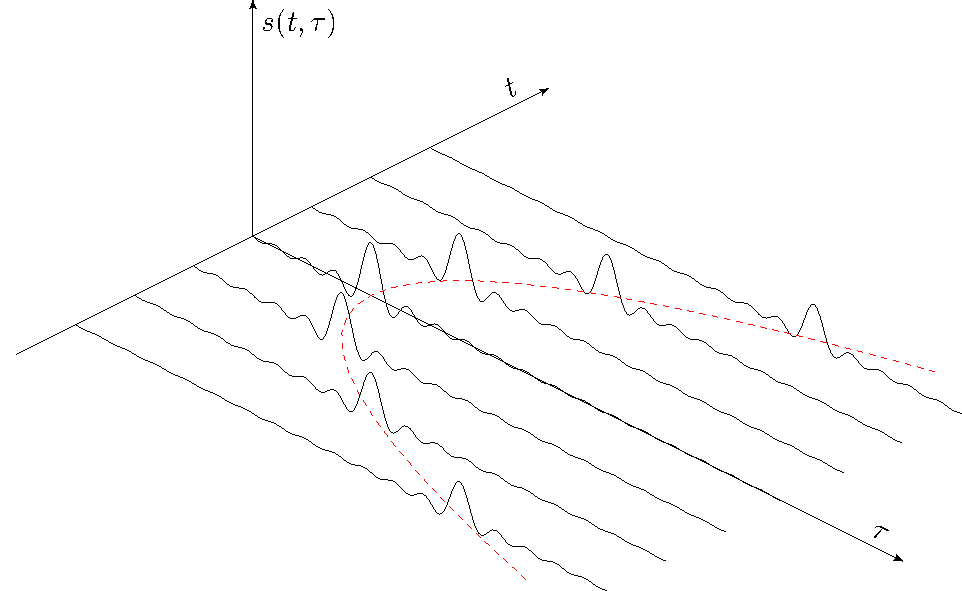
\includegraphics[width=13.5cm]{chapter2/echoes}
	\caption{雷达回波信号 ({\color{red}注意}:图注是五号字)} \label{fig_ch2_echoes}
\end{figure}

%-----------------------------------------------------------------------------------------
\BiSubsection{多幅图}{Multiple Figures}

如果一幅图中包含多幅子图,每一幅子图都要有图注,并且子图用 (a)、(b)、(c) 等方式编号,且各分图的分题注直接列在各自分图的正下方,总题注列在所有分图的下方正中,如图 \ref{fig_ch2_badge} 所示。
\begin{figure}[!ht]
	\centering
	\subfigure[灰色的交大校徽]{
\includegraphics[width=0.45\textwidth]{chapter2/xjtu_gray}} \hfill
	\subfigure[蓝色的交大校徽]{
\includegraphics[width=0.45\textwidth]{chapter2/xjtu_blue}}
	\caption{交大校徽 \label{fig_ch2_badge}}
\end{figure}

%=========================================================================================
\BiSection{表}{Tables} 

表格的设计应紧跟文述。表的编排一般是内容和测试项目由左至右横读,数据依序竖读,应有自明性。若为大表或作为工具使用的表格,可作为附表在附录中给出,论文中的表格参数应标明量和单位的符号。

表中各物理量及量纲均按国际标准(SI) 及国家规定的法定符号和法定计量单位标注。

表格要求采用三线表,与文字齐宽,顶线与底线线粗是 $1\frac12$ 磅,中线线粗是 1 磅。表格必须通栏,即表格宽度与正文版面平齐,如表 \ref{tab_ch2} 所示\footnote{{\color{red}注意}:图表中的变量与单位通过斜线 $/$ 隔开。}。
\begin{table}[!ht]
	\renewcommand{\arraystretch}{1.2}
	\centering\wuhao
	\caption{表题也是五号字} \label{tab_ch2} \vspace{2mm}
	\begin{tabularx}{\textwidth}{*{4}Y}
	\toprule[1.5pt]
		组号 & DOA / $^\circ$ & 带宽 / MHz & INR / dB \\
	\midrule[1pt]
		1 & $-30$ & 20 & 60 \\
		2 & 20 & 10 & 50 \\
		3 & 40 & 5 & 40 \\
	\bottomrule[1.5pt]
	\end{tabularx}
\end{table}

在三线表中可以加辅助线,以适应较复杂表格的需要,如表 \ref{tab_ch2_complex} 所示。

\begin{table}[!ht]
	\renewcommand{\arraystretch}{1.2}
	\centering\wuhao
	\caption{模态参数} \label{tab_ch2_complex} \vspace{2mm}
	\begin{tabularx}{\textwidth}{*{5}Y}
    \toprule[1.5pt]
    {$\textrm{方向}$}&{$\textrm{模态阶数}$}&{$\textrm{固有频率}\,/\,\mathrm{Hz}$}&{$\textrm{阻尼比}\,/\,\mathrm{\%}$}&{$\textrm{模态刚度}\,/\,\mathrm{N\cdot m^{-1}}$}\\
    \midrule[1pt]
    \multirow{2}{*}{$\mathrm{X}$}&1&500&2.11&1.2345$\times10^7$\\
    &2&800&3.11&1.3579$\times10^7$\\
    \cmidrule[1pt](l){1-2}
    \multirow{2}{*}{$\mathrm{Y}$}&1&500&3.11&1.5432$\times10^7$\\
    &2&900&5.11&1.2468$\times10^7$\\
	\bottomrule[1.5pt]
	\end{tabularx}
\end{table}

%=========================================================================================
\BiSection{公式}{Equations}

在 \LaTeX{} 中,行内公式用~$\$\ \ \$$~符号括起来。行间公式应另起一行,居中编排,较长的公式尽可能在等号后换行,或者在“+”、“-”等符号后换行。公式中分数线的横线,长短要分清,主要的横线应与等号取平。

公式后应注明编号,公式号应置于小括号中。写在右边行末,中间不加虚线。

公式下面的“式中:”两字左起顶格编排,后接符号及其解释;解释顺序为先左后右,先上后下;解释与解释之间用“;”隔开。

公式中各物理量及量纲均按国际标准(SI)及国家规定的法定符号和法定计量单位标注,禁止使用已废弃的符号和计量单位。

%-----------------------------------------------------------------------------------------
\BiSubsection{单个公式}{Equations}

\LaTeX{} 最强大的地方在于对数学公式的编辑,不仅美观,而且高效。单个公式的编号如式 (\ref{equ_ch2_pdf}) 所示,该式是正态分布的概率密度函数\citeup{Manolakis2005},
\begin{equation} \label{equ_ch2_pdf}
	f_Z(z) = \frac{1}{\pi\sigma^2} \exp\left(-\frac{|z-\mu|^2}{\sigma^2}\right)
\end{equation}
式中:$\mu$ 是 Gauss 随机变量 $Z$ 的均值;$\sigma^2$ 是 $Z$ 的方差。

%-----------------------------------------------------------------------------------------
\BiSubsection{多个公式}{Subequations}

多个公式作为一个整体可以进行二级编号,如式 (\ref{equ_ch2_fourier}) 所示,该式是连续时间 Fourier 变换的正反变换公式\citeup{Vetterli2014},
\begin{subequations} \label{equ_ch2_fourier}
	\begin{align}
		X(f) &= \int_{-\infty}^{\infty}x(t)e^{-j2\pi f t}\dif t \\
		x(t) &= \int_{-\infty}^{\infty}X(f)e^{j2\pi f t}\dif f
	\end{align}
\end{subequations}
式中:$x(t)$ 是信号的时域波形;$X(f)$ 是 $x(t)$ 的 Fourier 变换。

如果公式中包含推导步骤,可以只对最终的公式进行编号,例如:
\begin{align}
	\mbf{w}_{\mathrm{smi}} &= \alpha \left[\frac{1}{\sigma_n^2}\mbf{v}(\theta_0) - \frac{1}{\sigma_n^2}\mbf{v}(\theta_0) + \sum_{i=1}^{N} \frac{\mbf{u}_i^H\mbf{v}(\theta_0)}{\lambda_i} \mbf{u}_i\right] \nonumber \\
	&= \frac{\alpha}{\sigma_n^2} \left[\mbf{v}(\theta_0) - \sum_{i=1}^{N}\mbf{u}_i^H\mbf{v}(\theta_0)\mbf{u}_i +  \sum_{i=1}^{N}\frac{\sigma_n^2\mbf{u}_i^H\mbf{v}(\theta_0)}{\lambda_i} \mbf{u}_i \right] \nonumber \\
	&= \frac{\alpha}{\sigma_n^2} \left[\mbf{v}(\theta_0) - \sum_{i=1}^{N} \frac{\lambda_i-\sigma_n^2}{\lambda_i} \mbf{u}_i^H\mbf{v}(\theta_0)\mbf{u}_i \right]
\end{align}
